\documentclass[12pt,a4paper]{article}

% Margins.
\setlength{\oddsidemargin}{0in}
\setlength{\evensidemargin}{0in}
\setlength{\headheight}{12pt}
\setlength{\headsep}{0pt}
\setlength{\topmargin}{-60pt}
\setlength{\textwidth}{6.5in}
\setlength{\textheight}{10.75in}

\usepackage{amsmath}
\usepackage{float}
\usepackage{graphicx}
\usepackage[hyphens]{url}
\usepackage{hyperref}	% Clickable links to figures, references and urls.
\usepackage{datetime}
\usepackage{subfigure}

% Drawing.
\usepackage{pgf}
\usepackage{tikz}

% Listings for formatting code.
\usepackage{listings}
\usepackage{textcomp}
% General options.
\lstset{breaklines=true, basicstyle=\small\ttfamily, tabsize=4, numbers=left, stepnumber=1, frame=single, showstringspaces=false, upquote=true}
% C++ specific high-lighting. Comments are 50/50 shades of green/black and strings coloured with 60/40 red/black mixture.
\lstset{language=[ISO]C++, commentstyle=\color{green!50!black}, keywordstyle=\color{blue}, stringstyle=\color{red!60!black}}

%opening
\title{Electromagnetic Theory\\Assignment 03\\Line, Surface and Volume Integrals}
\author{Attique Dawood}
\date{September 22, 2014\\Due: September 26, 2014\\[0.2cm] Last Modified: \today, \currenttime}
\begin{document}
\maketitle
\noindent\textbf{Question 1:} Sketch and describe the following surfaces.
\begin{itemize}
\item[(a)] $\rho=2$
\item[(b)] $\phi=60^0$
\item[(c)] $r=5$
\item[(d)] $\theta=20^0$
\item[(e)] $\rho=1$, $0<\phi<\pi$ and $0<z<3$
\item[(f)] $r=1$, $0<\theta<\pi/2$ and $0<\phi<2\pi$
\item[(g)] $r=1$, $0<\theta<\pi/2$ and $0<\phi<\pi/2$
\end{itemize}
\noindent\textbf{Question 2:} A vector field is given by $\textbf{A}=2xyz\hat y$ in a region. Evaluate the flux, $\int\limits_{S}\textbf{A}\cdot d\textbf{S}$, through the surface given by $y=2$, $0<x<1$ and $2<z<5$.\\[0.2cm]
\noindent\textbf{Question 3:} Electric field of a point charge is $\textbf{E}=\dfrac{2}{r^2}\hat r$ in a region. Evaluate the flux, $\int\limits_{S}\textbf{A}\cdot d\textbf{S}$, through the spherical surface $r=1$.\\[0.2cm]
\noindent\textbf{Question 4:} Using $\int\limits_{a}^{b}\hat n\cdot d\textbf{\textit{l}}$
\begin{itemize}
\item[(a)] Find the arc length of a quarter circle of radius $\rho=3$ m in first quadrant.
\item[(b)] Find the length of the curve $y=x^2$ from (1, 1) to (3, 9). For this problem a calculator would be handy in solving the integrals.
\item[(c)] Find the length of the curve $y=2x^2+2$ from (0, 2) to (2, 10).
\end{itemize}
\noindent\textbf{Note:} For part (b) you need to find a unit vector along the curve $y=x^2$. A vector parallel (or tangent) to $y=x^2$ can be obtained from the slope. Numerator and denominator of slope ($\dfrac{dy}{dx}$) are the $y$-- and $x$--components, respectively, of the vector. Here, $\dfrac{dy}{dx}=\dfrac{2x}{1}$ so the parallel/tangent vector is $\textbf{n}=\hat x+2x\hat y$. The unit vector is then $\hat n=\dfrac{\hat x+2x\hat y}{\sqrt{1+4x^2}}$.\\[0.2cm]
\newpage
\noindent\textbf{Question 5 (Example 2--4C \cite[Example 2--4, page 23]{Cheng}):} Given a force field $\textbf{F}=xy\hat x+(3x-y^2)\hat y$ in a region, evaluate the integral $\int\limits_{P1}^{P2}\textbf{F}\cdot d\textbf{\textit{l}}$ to find the total work done by \textbf{F} in moving an object from P1 to P2 along path 1 and path 2.\\[0.2cm]
\noindent\textbf{Question 6:} Electric field in a region is $\textbf{E}=\dfrac{x\hat x+y\hat y}{(x^2+y^2)^{\frac{3}{2}}}$. Refer to figure \ref{Cheng-integral}, evaluate the integral $-\int\limits_{P1}^{P2}\textbf{E}\cdot d\textbf{\textit{l}}$ to find the potential difference between P1 and P2. Is the potential difference same for path 1 and path 2?
\begin{figure}[H]
\centering
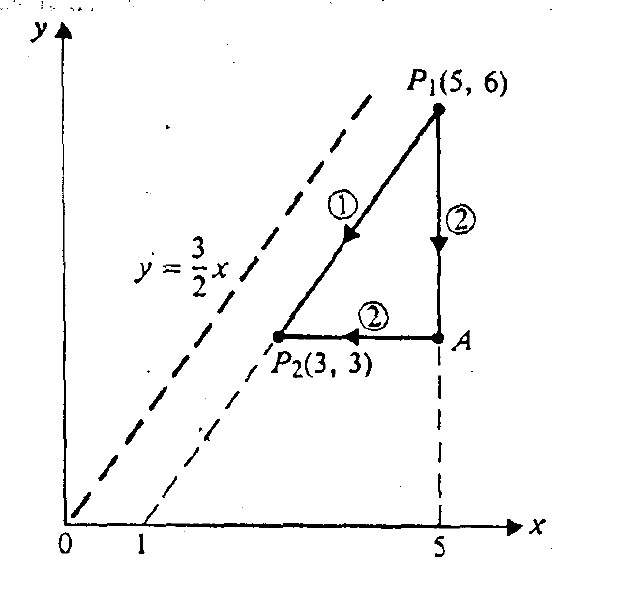
\includegraphics[scale=0.6]{Figure2-10Cheng.png}
\caption{Paths of integration for Questions 5 and 6 \cite[Figure 2--10, page 23]{Cheng}}
\label{Cheng-integral}
\end{figure}
\noindent\textbf{Question 7:} Refer to figure \ref{Circulation}. Electric field in the region is $\textbf{E}=\dfrac{x\hat x+y\hat y}{(x^2+y^2)^\frac{3}{2}}$.
\begin{itemize}
\item[(a)] Find $\oint\limits_L \textbf{E}\cdot d\textbf{\textit{l}}$ over the closed path ABCDA.
\item[(b)] Find $\oint\limits_L \textbf{E}\cdot d\textbf{\textit{l}}$ over the closed path ABCA.
\item[(c)] Find the potential difference between
\begin{itemize}
\item[(1)] A and B ($V_{AB}$).
\item[(2)] B and D ($V_{BD}$).
\item[(3)] A and C ($V_{AC}$).
\end{itemize}
\end{itemize}
\noindent\textbf{Note:} $V_{AB}=V_B-V_A=-\int\limits_{A}^{B}\textbf{E}\cdot d\textbf{\textit{l}}$.\\[0.2cm]
\noindent\textbf{Question 8:} Find the circulation of $\textbf{A}=\rho \cos\phi\hat \rho+\sin\phi\hat\phi$ over the path shown in figure \ref{Circulation}.\\[0.2cm]
\noindent\textbf{Question 9:} Do the following end--of--chapter problems from Sadiku \cite[Page 93 and 94]{Sadiku}: 3.1, 3.2, 3.3, 3.7, 3.8, 3.9 and 3.10.
\begin{figure}[H]
\centering
\mbox{
\subfigure[Path of integration for electric field given in Question 7.]{
\begin{tikzpicture}[xscale=1.2,yscale=1.2,font=\small]
	\def\XD{0cm}
	\def\YD{0cm}

	\draw[thick, ->, >=stealth] (1cm, 2cm) -- (2cm, 2cm);
	\draw[thick, ->, >=stealth] (2cm, 2cm) -- (2cm, 4cm);
	\draw[thick, ->, >=stealth] (2cm, 4cm) -- (1cm, 4cm);
	\draw[thick, ->, >=stealth] (1cm, 4cm) -- (1cm, 2cm);
	\draw[thick, ->, >=stealth] (2cm, 4cm) -- (1cm, 2cm);

	\draw[dashed] (0cm, 0cm) -- (1cm, 2cm);
	\draw[dashed] (0cm, 2cm) -- (1cm, 2cm);
	\draw[dashed] (0cm, 4cm) -- (1cm, 4cm);
	\draw[dashed] (1cm, 0cm) -- (1cm, 1.6cm);
	\draw[dashed] (2cm, 0cm) -- (2cm, 1.6cm);
	\draw[white,fill=white] (0.5cm,0.5cm) rectangle (1.5cm, 0.9cm);
	\node at (1cm, 0.7cm){$y=2x$};

	\coordinate[label=above:$C$] (C) at (2cm,4cm);
	\coordinate[label=above:$D$] (D) at (1cm,4cm);
	\coordinate[label=below:$A$] (A) at (1cm,2cm);
	\coordinate[label=below:$B$] (B) at (2cm,2cm);
	
	\coordinate[label=left:$2$] (y1) at (0cm,2cm);
	\coordinate[label=left:$4$] (y2) at (0cm,4cm);
	\coordinate[label=below:$1$] (x1) at (1cm,0cm);
	\coordinate[label=below:$2$] (x2) at (2cm,0cm);
	
	\draw[thick, ->, >=stealth] (0cm, 0cm) -- (0cm, 5cm);
	\coordinate[label=above:$y$] (y) at (0cm,5cm);
	\draw[thick, ->, >=stealth] (0cm, 0cm) -- (5cm, 0cm);
	\coordinate[label=right:$x$] (x) at (5cm,0cm);

\end{tikzpicture}
}
\quad\subfigure[Circulation of \textbf{A} for Question 8.]{
\begin{tikzpicture}[xscale=1.2,yscale=1.2,font=\small]
	\def\XD{0cm}
	\def\YD{0cm}

	\draw[thick, ->, >=stealth] (0cm, 0cm) -- (4cm, 0cm);
	\draw[thick, ->, >=stealth] (0:4)  arc (0:60:4) -- (0cm, 0cm);
	\draw[thick, ->, >=stealth] (0:4)  arc (0:30:4);
	\draw[thick, ->, >=stealth] (0:0.6) arc (0:60:0.6);
	\node[above] at (0.75cm, 0.2cm){$60^0$};
	
	\coordinate[label=below:$2$] (x2) at (4cm,0cm);
	
	\draw[thick, ->, >=stealth] (0cm, 0cm) -- (0cm, 5cm);
	\coordinate[label=above:$y$] (y) at (0cm,5cm);
	\draw[thick, ->, >=stealth] (0cm, 0cm) -- (5cm, 0cm);
	\coordinate[label=right:$x$] (x) at (5cm,0cm);

\end{tikzpicture}
}}
\caption{Circulation of vector fields.}
\label{Circulation}
\end{figure}
%\nocite{*}
\bibliographystyle{plain}
\bibliography{EMTRef}
\end{document}
